%------------------------------------------Packages used-------------------------------------------------
\documentclass[ebook, 12pt, twoside, openany]{memoir}
\usepackage[utf8x]{inputenc}
\usepackage[english]{babel}
\usepackage[top=4.5em,left=3.5em, right=3.5em, bottom=4em,footskip=1.4cm]{geometry}
\usepackage{titling}
\usepackage{adjustbox}
\usepackage{tabularx}
\usepackage{amsmath,amssymb,amsfonts,amsthm}
\usepackage{graphicx}
\usepackage{microtype}
\usepackage{enumitem}
\usepackage[listings,theorems]{tcolorbox}
\usepackage{hyperref}
\usepackage{xcolor}
\usepackage{setspace}
\usepackage{fancyhdr}
\usepackage{wrapfig}
%----------------------------------------------------------------------------------------------------------

\graphicspath{{images/}}
\hypersetup{
    colorlinks = true,
    urlcolor = blue!75!black,
    linkcolor = blue!70!black,
    }
\setlength{\parindent}{1em}
\setlength{\parskip}{1em}
\renewcommand{\baselinestretch}{1.75} 
\addto\captionsenglish{\renewcommand*\contentsname{Table of Contents}}
%-------------------------------------------------------
\title{{\textbf{Introduction to Nuclear Physics}}}
\vspace{2cm}  
\author{\textbf{Durjoy Dutta Chaudhury}}
%\predate{\centering}
\date{}
%\postdate{\vfill\hfill\emph{{\copyright Pradip Datta, Ananda Mohan College, Kolkata-700009}}\hfill}
%-------------------------------------------------------
\begin{document}
%-------------------------------------------------------

\maketitle
\pagebreak
\tableofcontents
%\listoffigures
%\listoftables

%----------------------------------------------------------------------------------------------------------
\pagestyle{fancy}
\fancyhf{}
\fancyhead[R]{\thepage}
\fancyhead[LE]{\tiny{\leftmark}}
\fancyhead[LO]{\tiny{\rightmark}}

\renewcommand{\headrulewidth}{1pt}

\fancypagestyle{the_end}{\fancyhf{}\renewcommand{\headrulewidth}{1pt}\fancyhead[R]{\thepage}
\fancyhead[LE]{\tiny{\leftmark}}
\fancyhead[LO]{\tiny{\rightmark}}\fancyfoot[R]{\textit{\tiny{}}}}


\thispagestyle{plain}
%-------------------------------------------------------------Chapter Inputs--------------------------------

    \chapter{Units \& Conversion}

\vspace{2cm}\begin{tcolorbox}
    [colframe=black!90!white,colback=yellow!29.05!white,arc=0.75em,fonttitle=\bfseries,title= \textit{Key Objective:}, width = \textwidth]   
        \begin{itemize}
        \item Atomic Mass Unit
        \item Unit Conversion
        \end{itemize}
    \end{tcolorbox}
   
   
\pagebreak\section{{Atomic Mass Unit}}
    Let us to calculate the coulomb barrier between two colliding nuclei! This can be a harrowing task (at least to me !) if we stick to our well known $SI$ unit system. It is to be noted that the $SI$ unit is convenient to express quantities used in daily life. However, it may not be suitable to express nucleons mass ($m_p=1.6726219×10^{-27} \ kg$), dimension ($10^{-15} \ m$) and other similar quantities related to atomic nuclei. Therefore, physicists introduced the concept of atomic mass unit ($a.m.u.$). since 1961, a unit of atomic mass is considered to be $\frac{1}{12} \ th$ of the mass of $^{12}C$ which is $12u$ ($u$ is the unit of mass). Note that there are a number of methods to determine the atomic mass and I advise you to consult any standard text book to learn those methods.\\
    \par We know that $1 \ gm \ mole$ of $^{12}C$ consists of Avogadro Number $(N_0)$ of atoms, i.e. $6.023×10^{23}$. Thus mass of one $^{12}C$ atom is ${12}/{N_0} \ gm$ or ${12×10^{-3}}/{N_0} \ kg$. Therefore, atomic mass $(u)$ in $^{12}C$ scale is 
    \begin{equation}
        \begin{split}
    u &= \frac{1}{12} × \frac{12×10^{-3}}{6.023×10^{23}} \ kg. \\[12pt]
    &= 1.660566×10^{-27} \ kg. \\[12pt]
        \end{split}
    \end{equation}
    \par Since we already know the $Mass$ \& $Energy$ equivalence principle, we express both $Mass$ in energy units by multiplying it with $c^{2}$. Hence
    \begin{equation}
         \begin{split}
    u &= 1.660566×10^{-27} × c^{2} \\[5pt]
    &= 1.660566×10^{-27} × 8.98755×10^{16} \ J \\[5pt]
    &= 14.924427×10^{-11} \ J \\[5pt]
    &= \frac{14.924427×10^{-11}}{1.60219×10^{-13}} \ MeV \\[5pt]
    &= 931.502 \ MeV 
         \end{split}
    \end{equation}
    \section{{Unit Conversion: Natural Units}}
    But do you notice the amount of jugglery between the units ! It is quite inconvenient if we need to go through these steps each time while solving numerical problems ! Let us go back to the problem we have already introduced: \textbf{\textit{The Coulomb barrier between two colliding nuclei.}}
    \par If we have to solve this problem with our SI unit approach, we need to solve the following equation (refer to the \href{https://en.wikipedia.org/wiki/Coulomb_barrier}{Wikipedia} page) as\\
    The electrostatic potential energy $(V_{Coulomb})$ is
    \begin{equation}
        \begin{split}
    V_{Coulomb} = k \frac{q_1q_2}{r} = \frac{1}{4 \pi \epsilon_0} \frac{q_1q_2}{r}~~~~~~~~~~~~~\\
            \textrm where,\\
            k~\textrm {is the Coulomb's constant}~= 8.9876×10^{9}Nm^{2}C^{-2};\\
            \epsilon_0~\textrm {is the permittivity of free space;}\\
            q_1,q_2~\textrm{are the chrages of the interacting nuclei;}\\
            r~\textrm{ is the interaction radius.}
        \end{split}
    \end{equation}
    
    This is quite frightening! Isn't it? Let us adopt a different approach. You need to remember the value only two fundamental quantities namely, the \textbf{Fermi Length} $(\hbar c)$ and the fine structure constant $\alpha$. \\
    \begin{equation}
         \begin{split}
          1. \ \hbar c \approx 197MeV.fm \\[12pt]
          2. \ \alpha = \frac{e^{2}}{4 \pi \epsilon_0 \hbar c } = \frac{1}{137}\\[12pt]
          \end{split}
    \end{equation} 
          
    Now let us rewrite $V_{Coulomb}$ with these inputs ! \\
    \begin{equation}
        \begin{split}
    V_{Coulomb} = \frac{\hbar c}{4 \pi \epsilon_0 \hbar c} \frac{q_1q_2}{r}
        \end{split}
    \end{equation}

    We replace $q$ with $q.e$. This way $q$ becomes just a number. Example: If you have $^{16}O$, $q_1$ is $16e$, where $e$ is the unit of charge. Therefore the above equation can be written as \\
    \begin{equation}
        \begin{split}
    &V_{Coulomb} = \frac{e^{2}}{4 \pi \epsilon_0 \hbar c} \frac{q_1q_2 \ \hbar c}{r} = \frac{197}{137} \ MeV. fm \ \frac{q_1q_2}{r} \\[12pt]
    &V_{Coulomb} = 1.44 × \frac{q_1q_2}{r} \frac{MeV.fm}{fm} = 1.44 × \frac{q_1q_2}{r} \ MeV. \\[12pt]
        \end{split}
    \end{equation}
    \par If we remember this little trick, we will be through many places in our course of $\emph{Nuclear Physics}$ at ease. \\[25pt]
%    \textcolor{red}{\textbf{H.W. \ Calculate the Coulomb barrier between $^{208}Pb$ \& $^{18}O$.}} \\[30pt]
    
\begin{comment}
    \begin{tcolorbox}
    [colframe=black!50!black,colback=white!100!white,arc=0.1em,fonttitle=\bfseries,title= \underline{Learning Outcomes:},width= \textwidth]
        \begin{itemize}
        \item $\textcolor{blue}{1 \ a.m.u. = 931.502 \ MeV}$
        \item \textcolor{blue}{Using the concept of fine structure constant and fermi length to handle numerical problems in \emph{Nuclear Physics} in a convient way. Example: Calculation of Coulomb Barrier between the colliding nuclei.}
        \end{itemize}
    \end{tcolorbox}
\end{comment}    

    \chapter{Nature of Nuclear Force}

    \begin{tcolorbox} [colframe=blue!10!black,colback=yellow!29.05!white,arc=1em,fonttitle=\bfseries,title= Key Objectives:, width = \textwidth]
        $\star$ \textbf{Origin of Nuclear Force} $\star$
        \begin{itemize}
            \item Strong Interaction(You may go through \\ \nameref{chap:funda})
        \end{itemize}
       $\star$ \textbf{Properties of Nuclear Force} $\star$ 
       \begin{itemize}
             \item Range (based on existing knowledge of Binding Energies) 
                \begin{itemize}
                    \item Short Range: Saturation Property
                    \item Repulsive Core: Concept of Incompressibility and Uniform Density of Nuclear Matter
                \end{itemize}
             \item Charge Independence and Charge Symmetric (Isospin)
       \end{itemize}
     \end{tcolorbox}
     
 \pagebreak   \section{Origin of Nuclear Charge}
            \begin{figure}
                \centering
                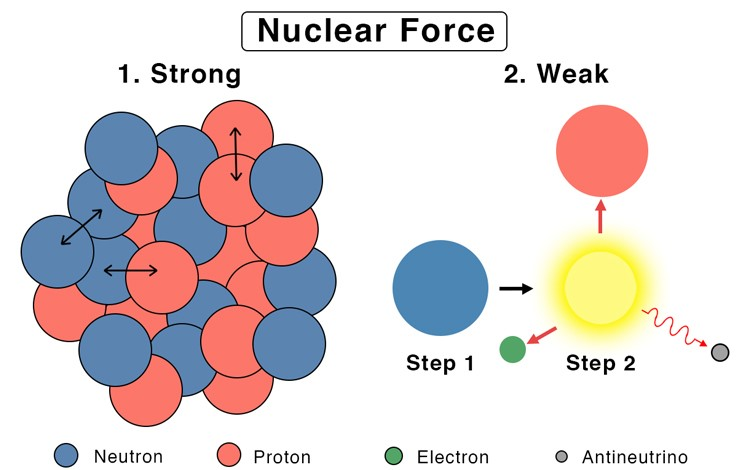
\includegraphics[width = 0.75\textwidth]{01/IMG4.jpg}
            \end{figure}
  The nuclear force (or nucleon–nucleon interaction) is a force that acts between the protons and neutrons and holds them inside the nucleus. In this class, we only need to know that the nuclear force is a residual effect of a fundamental force, namely the \href{https://en.wikipedia.org/wiki/Strong_interaction}{Strong interaction}. The Strong interaction binds the elementary particles known as \href{https://en.wikipedia.org/wiki/Quark}{quarks} which form the protons and neutrons.
      It is really fascinating how neutrons and protons are packed inside the tiny space \textit{(~few fm)} of a nucleus. Moreover, protons are positively charged and, hence, they must feel the tremendous repulsion due to Coulomb force. Thus, the nuclear force must be more powerful than the electromagnetic interaction (Coulomb interaction). However, in order to get more fundamental insight to our question of the nature of the nuclear force, we need to know a few basic things about the fundamental interactions in nature. Therefore, I request you to read the chapter \nameref{chap:funda}, if you are keen to know the underlying physics.\textit{ However, you may skip it for the time being and it will cause no harm to learn nuclear physics in its low energy domain. }

\section{Properties of Nuclear Force}
        $\bullet$~\textbf{Range:} Nuclear force is short range in nature and more powerful than the electromagnetic interaction. The nuclear force is extremely attractive between the nucleons at distances of about 1 fm. However, it decreases sharply beyond that and becomes insignificant beyond $\sim$ 2.5 fm. Due to this short range, a nucleon inside a nucleus can only interact with a few nucleons in its vicinity. This is known as the \textbf{Saturation property} of the nuclear force. Obviously, it must have come to your mind, how short is this ``Short range means"? This can be measured experimentally and even theoretically.
        
        \begin{wrapfigure}{r}{0.5\textwidth}
        %\centering
        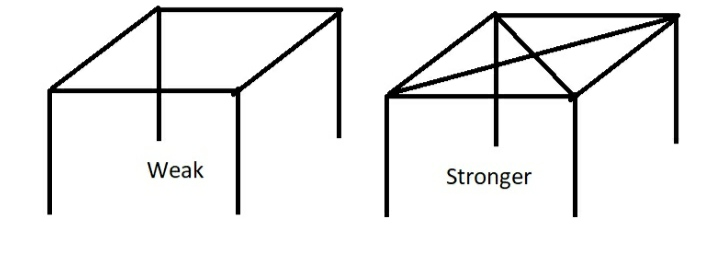
\includegraphics[width=0.5\textwidth]{01/IMG0.jpg}
        %\caption{\\Proton-neutron interaction}
        %\label{fig:nucleons}
        \end{wrapfigure}
        
$\star$~{\textbf{Read the following to have a better understanding of the short range nature of Nuclear Force: }}
\par Suppose you are building a house with bamboo sticks., you must have placed only four corner posts and connect them with one stick between each corner. At this time, your structure is not that strong. But as you keep on adding more and more connections (bamboos) between them, they become stronger and stronger. If you agree then let us analyse a nucleus.
 \par Replace the corners with nucleons (protons or neutrons) and the bamboos with the nuclear force.\textbf{ This model states that if we allow each nucleon inside a nucleus to interact with all the other nucleons inside it} then the heavier the nucleus, stronger the binding for each nucleon (imagine your Bamboo model).
         \begin{wrapfigure}{l}{0.5\textwidth}
        %\centering
        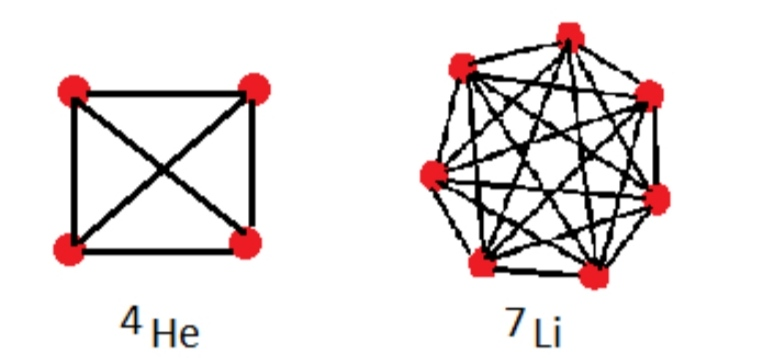
\includegraphics[width=0.5\textwidth]{01/IMG1.jpg}
        %\caption{\\Proton-neutron interaction}
        %\label{fig:nucleons}
        \end{wrapfigure}
Let us look at an example. In $^{4}He$, each nucleon has 3 connections and in $^{7}Li$ each nucleon has 6 connections. Thus, each nucleon in  $^{7}Li$ must be more strongly bounded than $^{4}He$. Similarly in $^{235}U$, there are 234 connections! Thus, B.E./A in $^{235}U$ should have been strongest. This can also be shown mathematically. If we consider the above assumption then a nucleus with A number of nucleons, can interact with A-1 other nucleons. So the total binding energy (B.E.) is proportional A(A-1)/2 (2 in the denominator to compensate for the double counting of the same pair of nucleons). If A is large, we may consider the B.E. is proportional $A^2$. Hence, B.E./A is proportional to A and B.E./A plot would be a monotonically increasing straight line graph. But, this is not what we have learnt from the B.E./A plot (B.E./A is nearly constant and it is around 8 MeV).

The above analysis tells us that nuclear force is  short range. Therefore, a nucleon can only interact with a few nearby nucleons. Therefore, B.E. is not proportional to A.(A-1) but proportional to A. Hence, B.E./A is constant which is a direct consequence of the short range nature of the nuclear force. 

        $\bullet$~\textbf{Hard Core:} In order to prevent the nucleus from collapsing from the tremenduous powerful attraction, a repulsive component exists in the nuclear force. This short-range repulsive force becomes very large and repulsive for separations less than about 0.7 fm.
        \begin{wrapfigure}{r}{0.5\textwidth}
        %\centering
        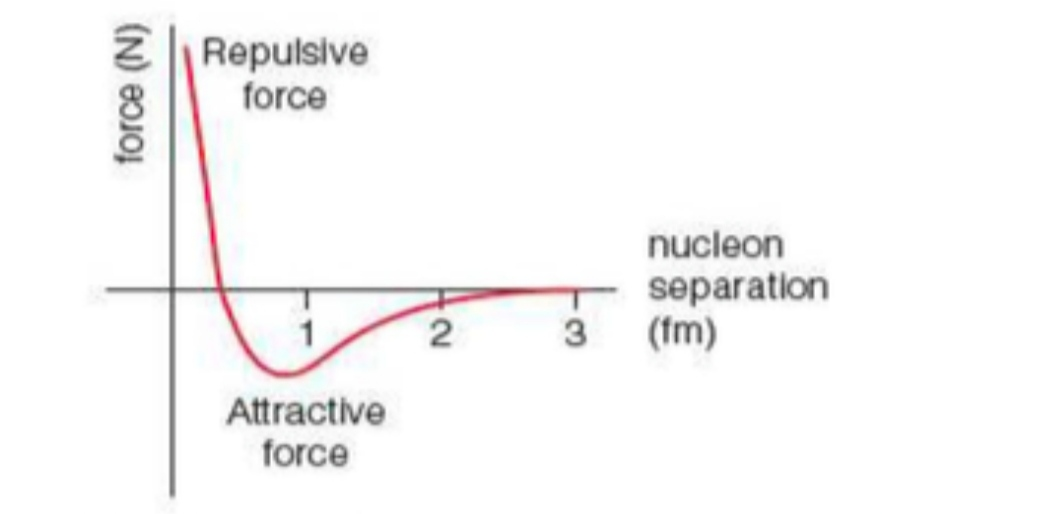
\includegraphics[width=0.5\textwidth]{01/IMG2.jpg}
        %\caption{\\Proton-neutron interaction}
        %\label{fig:nucleons}
        \end{wrapfigure}
        The adjacent figure shows the results of the superposition of the short range attractive and the repulsive force components. Thus, it maintains the similar average separation between the nucleons in all nuclei.\textbf{ It leads to the uniform density of nuclear matter ($\sim~2.3×10^{17}$ kg/m3) and will be used to calculate the radius of a nucleus.}   
        
        $\bullet$~\textbf{Charge Symmetric \& Charge Independence:} Experiments show that Nuclear Force is not affected bu Coulomb interaction. Therfore, it is the same between two protons or neutrons inside a nucleus. Of course, the Coulomb repulsion has not been taken into account. This is known as charge symmetry of nuclear force and symbolically:
        \begin{equation}
            (n-n)~=~(p-p)
        \end{equation}
Thus,  the force between a proton and neutron should be the same as the above. Hence,
        \begin{equation}
            (n-n)~=~(p-p)~=~(p-n)
        \end{equation}
 
         \begin{wrapfigure}{l}{0.55\textwidth}
        %\centering
        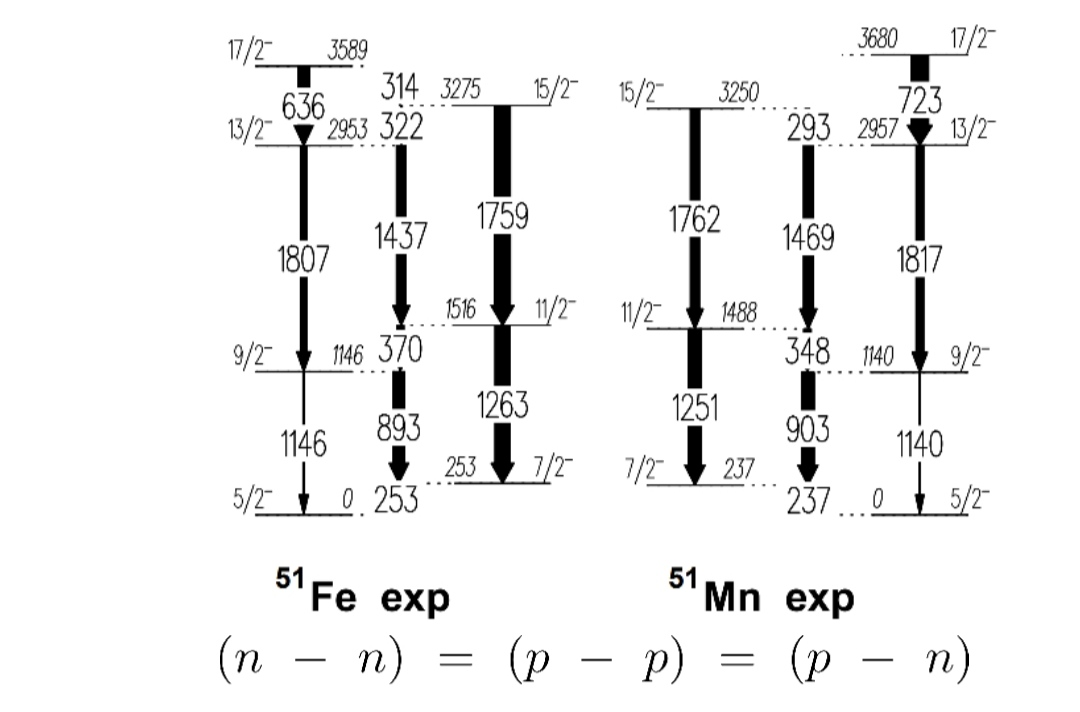
\includegraphics[width=0.55\textwidth]{01/IMG3.jpg}
        %\caption{\\Proton-neutron interaction}
        %\label{fig:nucleons}
        \end{wrapfigure}
This is called charge independence. Thus, inside a nucleus, the charge symmetry is broken by the electromagnetic interaction due to the charge of the proton. The validity of this hypothesis is substantiated with the striking similarity in the excitation spectra of \href{https://en.wikipedia.org/wiki/Mirror_nuclei}{mirror nuclei} and in the n-n, n-p and p-p scattering experiments.


\par$\bullet$~\textbf{Isospin:} Based on the above concept a hypothesis was introduced (before the quark came into the picture) where proton and neutron are considered as two different states of a nucleon. The nucleon-nucleon force is the same irrespective of whether the nucleons are protons or neutrons - once the coulomb repulsion has been taken out. Hence, we can introduce a new quantum number, Isospin, similar to that of electron spin (S), to define two states, one for protons and the other for neutrons. We assign an isospin value of 
\begin{equation}
   \tau = 1/2
\end{equation}(in the same way, as we assign   for S = 1/2 electron spin). In low-energy nuclear physics, we chose the isospin projection
\begin{equation}
   \tau_z = 1/2
\end{equation}
for neutrons and
\begin{equation}
\tau_z = -1/2
\end{equation}
for protons  which are opposite in particle physics.  

    
\par\textbf{\underline{Note:}} \textit{It is to be noted that even after almost 100 years of our best efforts, understanding of the nuclear potential is still incomplete. The primary problem is that the experimental data suggest that there is a three body interaction component in the nucleon-nucleon interaction. Such interaction among a finite number of particles requires advanced mathematical techniques and moreover computational support to handle such large scale calculation. This is a front-end research domain and till date successful for nuclei up to  $A=12$.}      
          
    \chapter{Fundamental Interactions}
\label{chap:funda}
    \begin{tcolorbox} [colframe=blue!15!black,colback=yellow!29.05!white,arc=1em,fonttitle=\bfseries,title= Key Objectives:, width = \textwidth]
        $\star$ \textbf{Fundamental Interactions in Nature} $\star$
        \begin{itemize}
            \item Strong Interaction
            \item Weak Interaction
            \item Electro-Magnetic Interaction
            \item Gravitational Interaction
        \end{itemize}
       $\star$ \textbf{Force Carriers} $\star$ \\
       $\star$ \textbf{Feynman Diagram} $\star$
       
     \end{tcolorbox}
    
    \section{Fundamental Interactions}
 We may have experienced so many different types of forces around us but the amazing
simplifications in physics is that only four fundamental interactions can account for all known physical phenomena happening around us in the \href{https://en.m.wikipedia.org/wiki/Standard_Model}{{{Standard model}}}.
These four interactions have different ranges, different strengths and act in completely different time and mass scales. 
The summary of these four fundamental interactions are as follows: \\
  
\begin{table}[ht]
        \centering
        \begin{adjustbox}{width=1\textwidth}
        {\Large
        \begin{tabular}{|l|l|c|c|c|p{5cm}|}
            \hline
            \textbf{Interaction} & \textbf{Force Carrier} & \textbf{Relative Strength} & \textbf{Range(m)} & \textbf{Nature} & \textbf{Example}\\[0.5cm]
            \hline
              
            \textbf{Gravitational} & \textbf{\emph{Graviton}} & $10^{-38}$ & $\infty$ & \textbf{Attractive} & {Interaction due to mass} \\[1.25cm]
              
            \textbf{Electro-magnetic} & \textbf{\emph{Photon}} & $10^{-2}$ & $\infty$ & \textbf{Attractive/Repulsive} & {Interaction due to Charge} \\[1.25cm]
              
            \textbf{Weak} & \textbf{\emph{Vector Bosons} \newline ($W^\pm,Z^0$)} & $10^{-5}$ & $10^{-18}$ & \textbf{Attractive/Repulsive} & {Change of the flavour \newline of Quark i.e Beta-decay} \\[1.25cm]
              
            \textbf{Strong} & \textbf{\emph{Gluon}} & $1$ & $10^{-15}$ & \textbf{Attractive/Repulsive} & {Interaction between Quarks}\\[1.25cm]\hline
    
    \end{tabular}}
    \end{adjustbox}
\caption{Summary of fundamental interactions}
\label{tab:table_1}
\end{table}
    
    \par You must have been quite uncomfortable with so many new terms such as Quarks, Vector Bosons, Gluons and flavour. Don't worry we will learn about them in due course of time but for the time being let us concentrate only on the interactions.
    \pagebreak\begin{itemize}
          \item\textbf{The strong interaction} is the strongest among all the four. It acts over an extremely short range and thus loses its superiority beyond a few \textit{fermi}. It determines the stability of nuclei and thus relative abundance elements in nature. The properties of the nucleus also determines the number of electrons in it and therefore, indirectly controls the chemical reactions. It also determines the release of energy in nuclear reactions.
          \item\textbf{The Electro-magnetic interaction} is a combination of electric and magnetic force.(Till the beginning of the 19th century, these two were considered as two distinct forces. Riding on the series of works of various scientists between 1820 and 1873, James Maxwell formally unified these two seemingly different forces into one as electromagnetic interaction). It is a long-range force and it acts over extremely large distances. Though it is the second strongest interaction among the four and responsible for almost all phenomena(eg. friction, tension, chemical reactions and electrical effects) we experience in our daily lives. However, its often cancels out in the macroscopic body and becomes insignificant. However if it does not cancel, it would supersede the Gravitaional Force as expected.
          \pagebreak\item\textbf{The Gravitational interaction} is the weakest among the four partners and is always attractive. But it is interesting to note that it is the key interaction which determines the evolution of the universe once the matter is formed. In astronomical scale, it dominates over the other interactions and as we know it, governs the motions of the celestial objects. The gravitational force is also responsible for modifying the space and time near very massive bodies, such as stars and planets.
        \end{itemize}
        
    \section{Force Carrier/ Exchange Particles}
    One thing must have come to your mind, ``How can two particles interact with each other without any physical contact?'' or ``How does a charged particle know that there is(are) other charged particle(s) in another location(s)?"
    
    \par Here comes the concept of a force carrier. It was first proposed by Yukawa's in 1935 while working on the nuclear force.(Earlier, Heisenberg had applied the concept of exchange force to explain the formation of $H_2$ molecules through the binding of Hydrogen atoms.) Yukawa proposed that the interactions are transmitted by the exchange of elementary particles. Note that this concept complements the concept of force field. According to the force field concept, the interactions between two particles maybe described as a field generated by each particle which affects others due to the exchange of field quanta. When we quantize these  fields, it results in various excitation states and each state corresponds to a different generation of force carrier particles (we will discuss this ``different generation of force carrier particles", in the Fundamental particles section.) If not for the other interactions, the field is called the Electromagnetic Field and the particle is, Gluon. The other exchange particles for the other interactions are given in the above table. We will conclude this paragraph mentioning that these force carrier particles are considered as Virtual Particles. In the next paragraph, we will explore this term and see how we can even violate conservation of mass-energy principle. Yes! you hear it correctly. Let us start:
    
        \par {\textbf{Virtual Particle: } Suppose, you have a particle with energy $E$. The Heisenberg Uncertainty Principle states that this energy cannot be measured with any arbitrary accuracy. If you want to measure it with an accuracy of $∆E$, you need to make this measurement over a time interval greater than $\hbar/∆t $ (using $\Delta E \Delta t > \hbar $). So, we don't know what is happening within the time interval $\Delta t$. It is gone to the extent that even if we violate the well known mass-energy conservation by an amount $\Delta E $, then by no means anybody can detect this violation within the time gap $\Delta t $. Therefore, it is possible to create a temporary field quanta of mass m($=c^2/\Delta E$) for a time interval of $\Delta t $. These field quanta are called Virtual Particles as they don't live beyond $\Delta t $ and thus cannot be directly observed. However we can record their effects. }
         \par [
         \textbf{\underline{Note:}} \textit{Virtual particles are real particles. According to Quantum Mechanics, every particle spends some time as a combination of other particles in all possible ways. It is well established and tested. Though the virtual particles are temporary, they interact with real particles and leave their `fingerprint' which can be experimentally verified unambiguously. The first proof was the observation of the Lamb Shift in Hydrogen atom by Willis Lamb and fir which he won the Nobel Prize.}]
         
         \par{\textbf{Range of the Interaction:} The above concept also allows us to estimate the range of the interactions. We have learned that Exchange Particles or Field Quantas are temporary and exist only for $\Delta t $. We can extend it to another step as     \begin{equation}
                \Delta t = \hbar/ \Delta E = \hbar/mc^2
            \end{equation} 
         If we consider the exchange particles are massive, then heavier their mass, shorter their existence $\Delta t $. If we further assume their velocity is equal to speed of light $c$ then in time $\Delta t $, it can travel a distance $r_0$, called range.}
             \begin{equation}
             r_0 = c. \Delta t = c \hbar/mc^2 = \hbar /mc
             \end{equation}
         \par Let us look at the implication of this concept. We already know that the strong interaction is very short range and radius of any nucleus is order of few \textit{fm}. Then
         \begin{equation}
         \begin{split}
                    mc^2~\sim~\hbar c /r_0 = 197/2 (MeV~fm)/fm =100~MeV
                    \\\textrm (assuming~~r_0 \sim 2fm)
         \end{split}
         \end{equation}
        \par This way Yukawa predicted the mass of the Mesons ($\pi^\pm , \pi^0$ to be $~$100 MeV. Later it was found to be $~$139 MeV and if you agree this is remarkable.
        
        \begin{wrapfigure}{r}{0.45\textwidth}
        \centering
        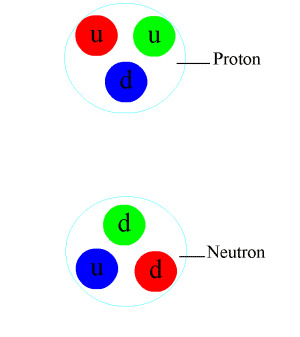
\includegraphics[width=0.3\textwidth]{02/nucleons.jpg}
        %\caption{\\Proton-neutron interaction}
        \label{fig:nucleons}
        \end{wrapfigure}
        
    Now you should realize why Electromagnetic Interaction is long range (infinite range). It is due to the fact that its exchange particle, Photon, is massless. This way we can predict the mass of the exchange particles if we know the range of the interactions or vice–versa. The attached animation (source: \href{https://en.wikipedia.org/wiki/Nuclear_force}{Wikipedia} ) portrays the interaction between a proton and a neutron through the exchange of a Meson.

    \par The process described above can also be visualized in pictorial form. It was first proposed by Richard Feynman. Though we have no intention to learn it in full glory which is beyond the scope of this class, we just like to get a taste of it. 
    
    \section{Feynman Diagram}
        \par We have learned that for each interaction there are virtual particles which exist only for $\Delta t $ time interval. Therefore, we can exploit this uncertainty to formulate a picture of the particle or particles in question in a space-time diagram. For sake of simplicity, we consider an electron at rest. If the electron emits a photon and absorb the same with a time interval of $\Delta t $, we won't be able to realise that. Such an event can be drawn as follows: 
        \par The Fermions are represented by a straight line with an arrow directing the flow of the particle. The photons are represented by a wavy line. The points where particles are created or annihilated are called Vertices. Here the line is vertical as the electron is at rest and only time is changing. During the time interval $\Delta t(= t_2–t_1)$, the virtual photon is created at $t_1$
        \begin{figure}
            \begin{center}
                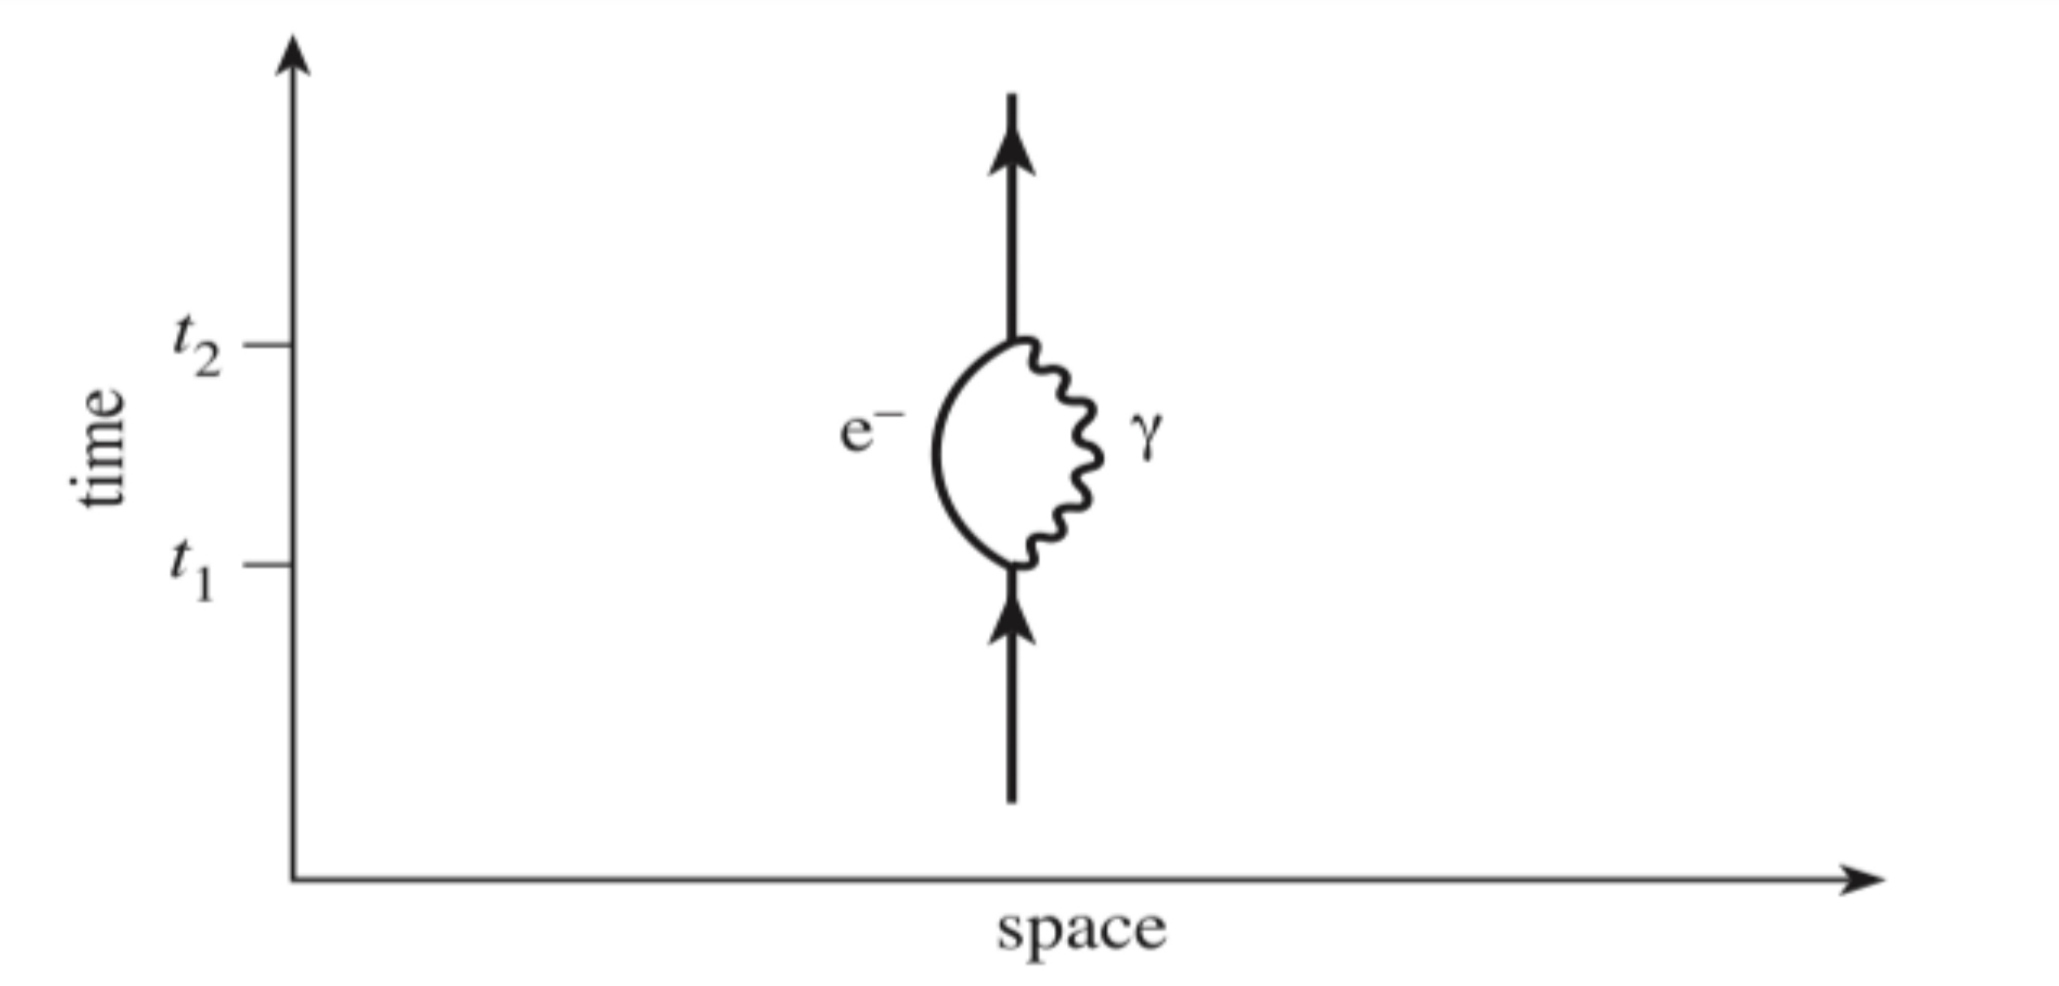
\includegraphics[scale=0.10]{02/img1.jpg}
            \end{center}
            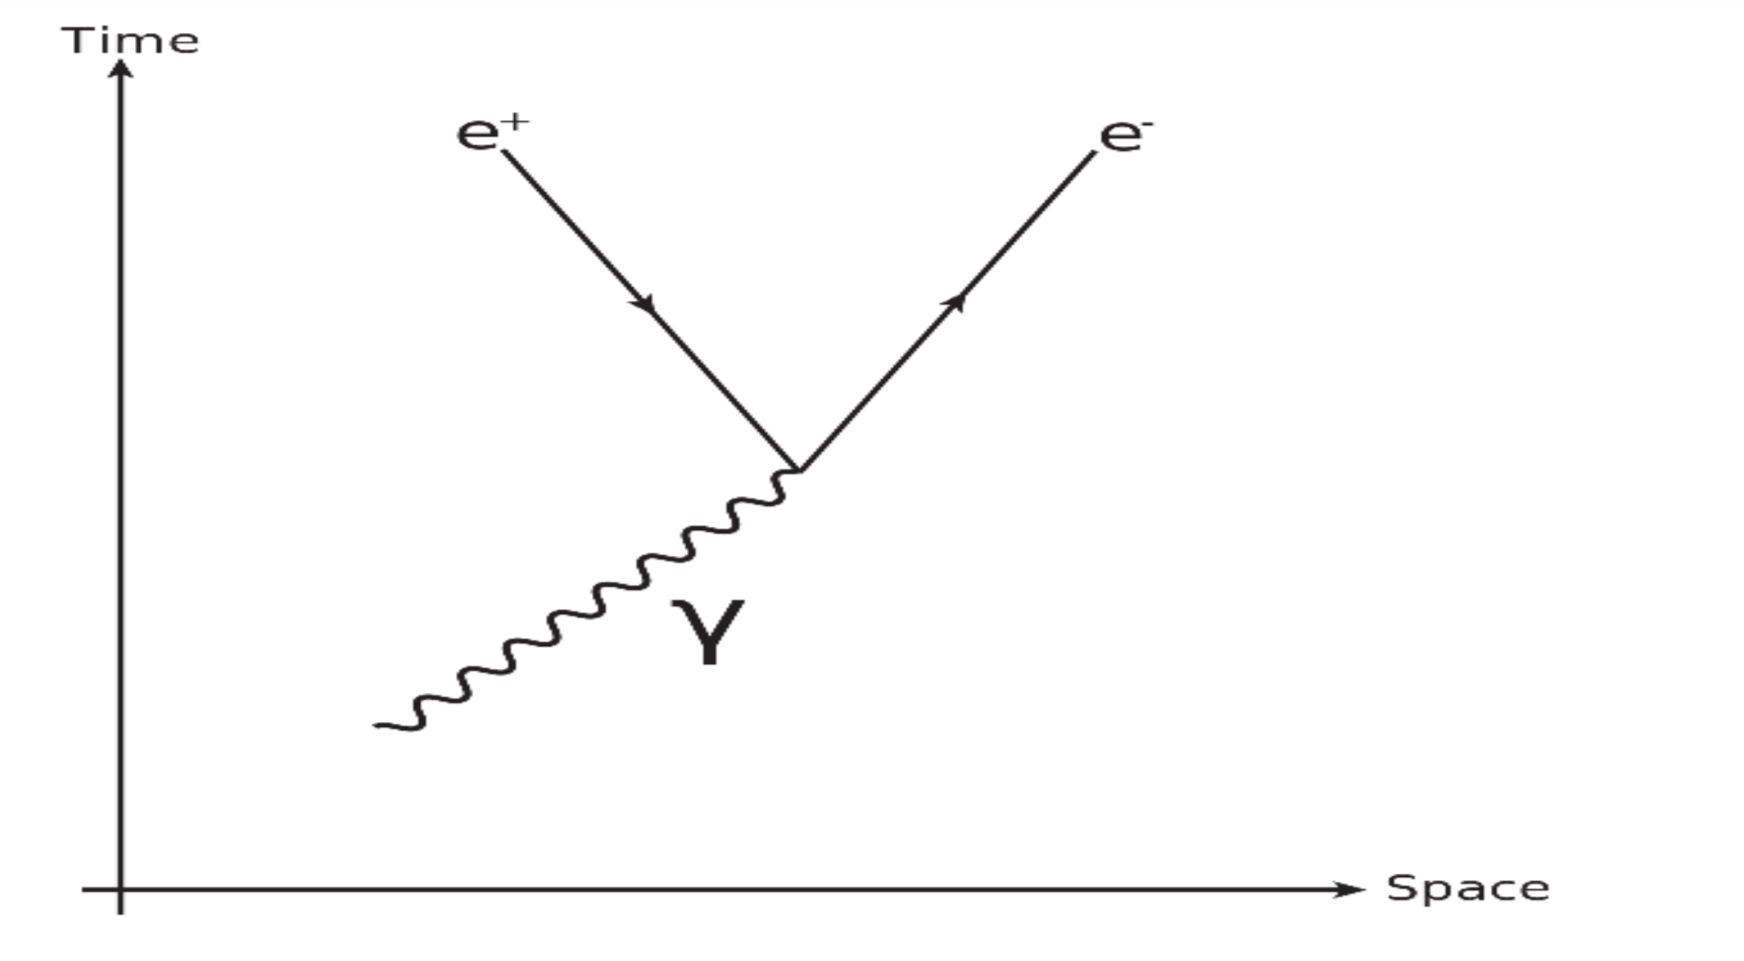
\includegraphics[scale=0.10]{02/img2.jpg}
            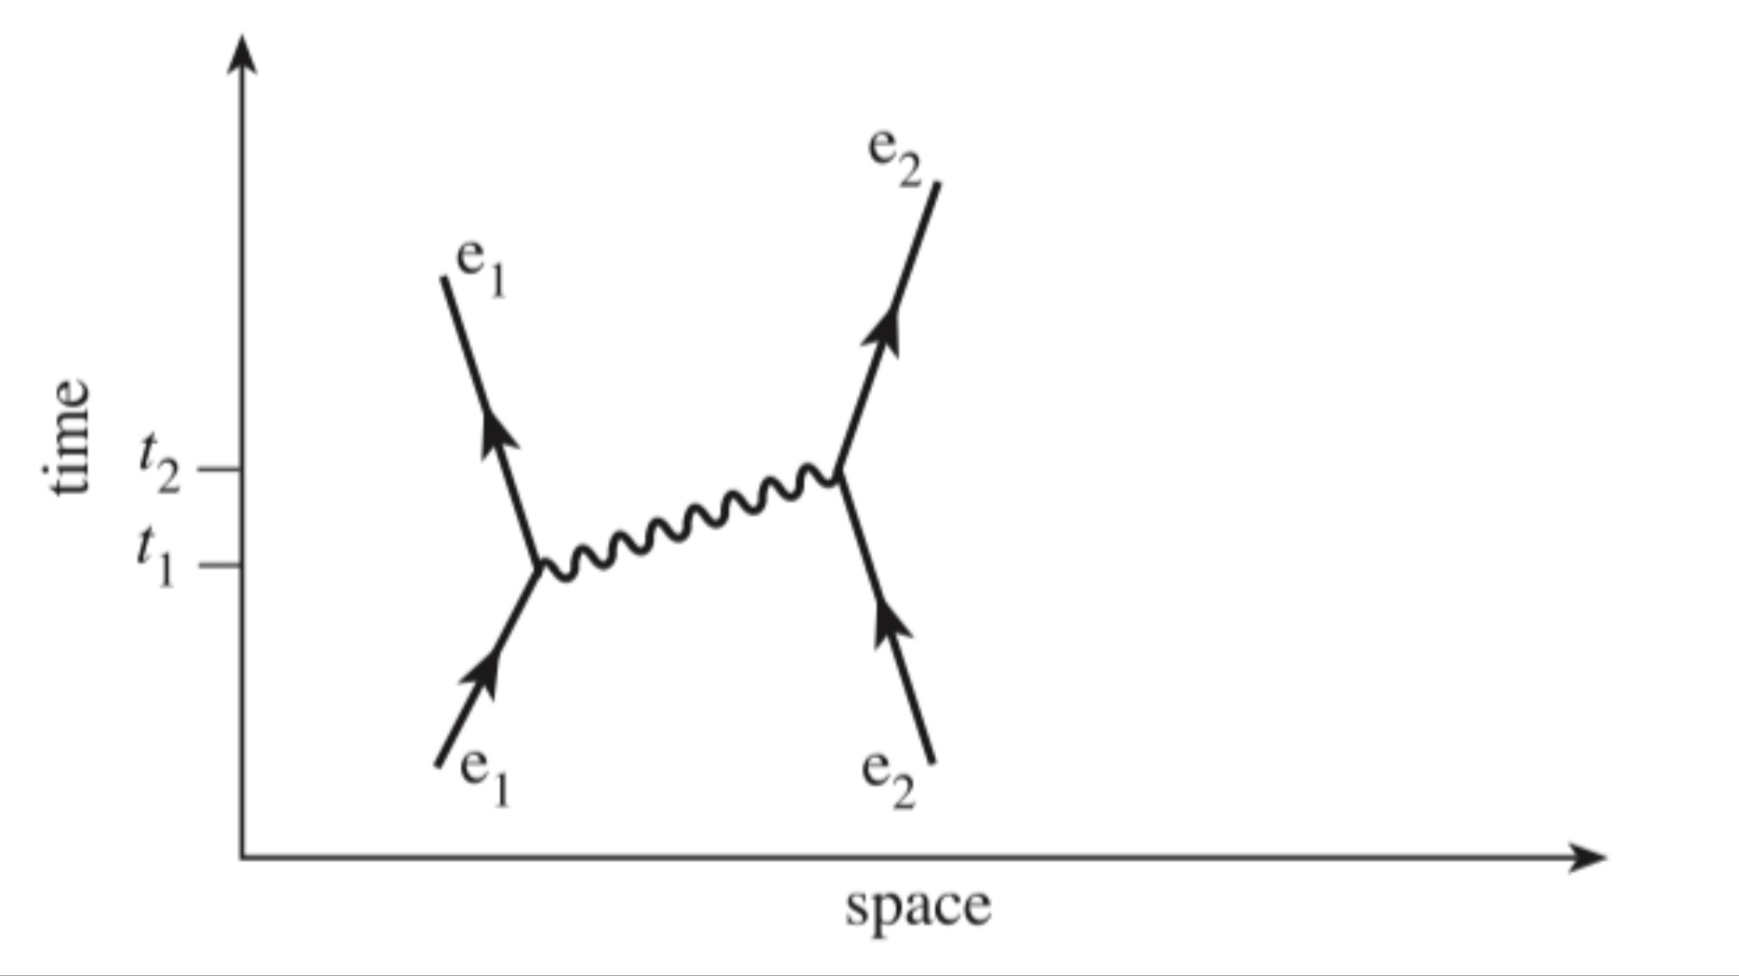
\includegraphics[scale=0.10]{02/img3.jpg}
            \caption{Feynman diagrams}
            \label{fig:plot_time_space}
        \end{figure}
        and once again absorbed at $t_2$. Similarly, the process of pair production can be represented by the above diagram. Note that the arrow of an anti-particle will be drawn backwards in time (opposite of particle). Two electrons scattering may be represented by the following figure:  At $t_1$, electron $e_1$ emits a virtual photon and to conserve momentum it will recoil to the left. At $t_2$ ($<\Delta t$), $e_2$ absorbs the photon and deflects to the right to conserve momentum. In addition, the total energy of the two–electron system should remain the same before and after the scattering to satisfy the energy conservation principle.
 
    \chapter{Liquid Drop Model}

\begin{tcolorbox} [colframe=blue!10!black,colback=yellow!29.05!white,arc=1em,fonttitle=\bfseries,title= \textit{Key Objective:}, width = \textwidth]
$\star$ \textbf{Liquid Drop Model} $\star$
\begin{itemize}
    \item Nuclear Landscape
    \item Liquid drop model
    \item Similarities \& limitations
    \item Bethe–Weizsäcker mass formula \\ (Semi-empirical mass formula) 
\end{itemize}
\end{tcolorbox}

\pagebreak\section{Nuclear Landscape}
Our knowledge of the nuclear force gives us understanding about the formation of nuclei. There are about 3300 nuclei known to us but only a fraction of them are stable! In fact, it is around only 15\% of the total list. Most of the unstable (radioactive) nuclei undergo -decay and few, mostly the heavy nuclei decay through  particle emission. Some of the heavy nuclei also undergo spontaneous fission (breaking of a nucleus into two lighter nuclei). This can be clearly seen in the Z vs N plot from figure \ref{fig:plot_ZvsN} which is also known as Segre chart (\href{https://www.nndc.bnl.gov/nudat2/}{link for more info.}) of all the known nuclei.



\par The black dots in the plot are the stable nuclei whereas the other colours correspond to unstable nuclei with varying half-life (range is given in the box). It shows that as we move toward the heavier nuclei, it needs more neutrons than protons to stabilize a nucleus. This observation seemingly contradicts the charge symmetry of the nuclear force! However, it may be explained as the effect of Coulomb repulsions between the protons which weaken the binding energy of a nucleus. To compensate for this loss, more and more neutrons are needed in heavier nuclei. At this point if we recollect our lessons from B.E./A systematics,


    \pagebreak\begin{figure}
                \centering
                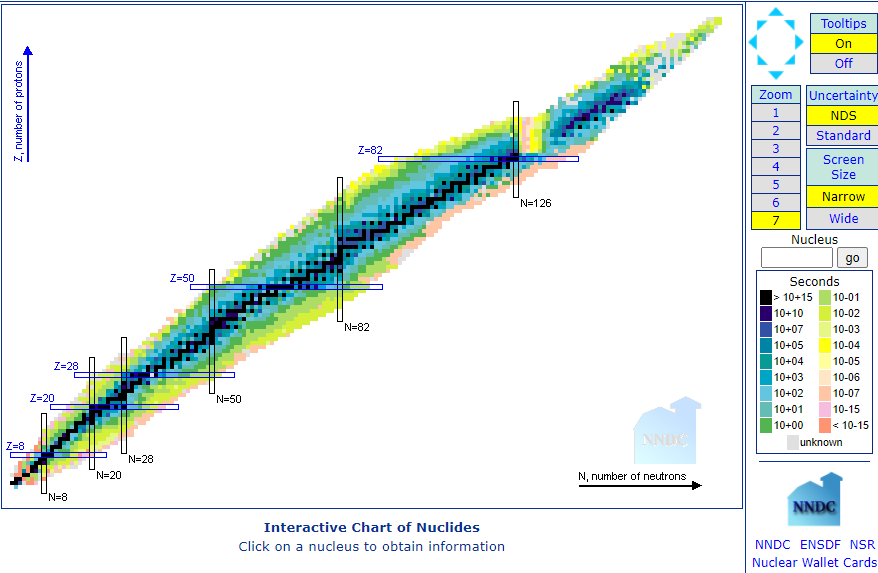
\includegraphics[width = 0.9\textwidth]{03/ZvN_plot.png}
                \caption{Z vs N Plot}
                \label{fig:plot_ZvsN}
            \end{figure}

we have seen that even-even (both N and Z are even) nuclei are strongly bound compared to their odd-odd neighbours with same A (isobar). Similarly, for isotopes (nuclei with same Z) and isotones (nuclei with same N), it has been observed that odd-even or even-odd combinations are relatively stronger bound than neighbouring odd-odd combinations and weakly bound with respect to even-even neighbours. This tells us apart from the attractive short range interaction and Coulomb force, there are other components in the nuclear force. In this class, we will develop a phenomenological (Semi-empirical) model of the nucleus as functions of A, Z and N using existing knowledge of the nuclear force and features of binding energy.



\par The above discussion must have triggered an intriguing question in your mind: what is the difference between an even-even and an odd-odd nucleus from the nuclear force aspect? In fact there should not be any! The answer lies in the fact that the exact form of the nucleon-nucleon interaction is still not known to us. There are many components in it and not necessarily all of them will help in increasing binding energy of a nucleus. It is further to be noted that even if we know the exact form of the potential, we can not solve the corresponding Schrodinger equation exactly due to the presence of three body components in the nucleon-nucleon interaction to a many body system. Exactly at this point the nuclear physics, low energy nuclear physics to be precise, differs from the atomic physics which can be solved exactly with the electro-magnetic interaction which is exactly known to physicists. This led to the development of a model to explain the observed features. The known properties of the nuclear force will act as the input to the model.


    \subsection{$\star$ What is a model in science?}
 A scientific model is a conceptual representation of a system to understand, visualize, or simulate the system using the accepted knowledge. Usually, a model is bound by strict assumptions and intends to describe a few particular features of the system. Therefore, no model intends to give a full description of the system from all angles but to explain a few features. 

%\pagebreak

\section{Liquid Drop Model}
This model was first proposed by N. Bohr and F. Kalcker in 1937. Later it was refined and applied by C. F. von Weizsäcker and H. Bethe to develop the semi-empirical mass formula (also known as \textbf{Bethe–Weizsäcker mass formula}) as mentioned above.  The model has been very useful for the understanding of nuclear fission data and predicting the masses and stability of a nucleus based on the Strutinsky method. The analogy between the charged liquid drop and atomic nucleus can was made based on the following similarities:

    \begin{itemize}
    
        \item Similarities:
        
            \begin{enumerate}
                \item Like nucleons, molecules in liquid drop also interact with the other molecules in their immediate neighbourhood. Therefore, the interaction between the molecules in a liquid also exhibits saturation properties. Thus, the number of molecules (A) in a liquid drop $\propto$ its volume (V). This can be alternatively established as the total heat required to evaporate a drop of liquid is linearly proportional to the number of molecules in the drop. It is analogous to the total binding energy of a nucleus which is proportional to the number of nucleons in that nucleus.
                \item Like nucleons, the intermolecular force in a liquid is repulsive at short distances and attractive at intermediate distances and negligible at large distances.
                \item Like a nucleus, a liquid drop is also nearly incompressible.
                \item Nucleons near the surface of the nucleus feel less interaction like the surface tension effects observed in liquid drop.
                \item The internal energy of a nucleus is analogous to the internal thermal vibrations of molecules in the liquid.
                \item Emission of $\alpha$, $\beta$, p and n may be compared with the evaporation of molecules from liquid.
            \end{enumerate}
        
        \item Limitations:
            \par It is to be noted that there are also striking similarities between a charged liquid drop and an atomic nucleus (which must be quite obvious to you). These are as follows:
        
            \begin{enumerate}
                \item The foremost difference is that the motion of the nucleons inside a nucleus is of quantum mechanical character whereas the motion of molecules in a liquid is classical in nature.
                \item Intermolecular attraction acts beyond the dimensions of the electron shells. They also strongly repel each other once the distance is smaller than the size of the electron orbits. On the contrary, nuclear force is attractive within the smaller range, the range of the nuclear forces.
                \item The average kinetic energy of the molecules in the liquid is $\sim0.1$ eV which corresponds to the de-Broglie wavelength of $\sim10^{-11}$ eV. The average kinetic energy of the nucleons in nuclei is $\sim10$ MeV and it corresponds to the de-Broglie wavelength $\sim10^{-15}$ m order of inter-nucleon distances.
            \end{enumerate}
    \end{itemize} 
    
Based on the above similarities between the charged liquid drop and atomic nucleus, the liquid drop model was developed. We know that the binding energy ($E_B$) of a nucleus with atomic mass M(A, Z) may be written as
    \begin{equation}
    E_B = ZM_H + NM_n - M(A, Z)
    \end{equation} 
\par In a phenomenological model, we add different components by hand based on our experimental observation. Let us approach in the same way with our knowledge about $E_B$ as follows:


\begin{enumerate}[label=\textbf{\Alph*.}]

    \item \textbf{Volume term:}     If we apply our knowledge of nuclear force, the most powerful component would be the attractive short range nuclear force which is proportional to the volume of the nucleus. This term, known as volume energy ($E_v$), obviously favours the binding energy and, thus, is considered positive. It may be written as
        \begin{equation}
            \begin{split}
                E_v &\propto V\\
                E_v &\propto A = a_VA
            \end{split}    
        \end{equation}
        where $a_V$ is the constant of proportionality.

    \item \textbf{Surface term:}    Each nucleon interacts with a fixed number of nucleons and it is independent of A. This is the core concept of the volume energy term. However, this is not true for the nucleons on the surface of the nucleus which have less number of neighbouring nucleons. Therefore, the second term, which is known as the surface energy ($E_s$), is a correction to the volume term and should be subtracted from the volume term. It is proportional to the surface area of the nucleus and can be written as:
        \begin{equation}
            \begin{split}
                E_s \propto -4\pi R^2 &\propto -4 \pi (r_0A^{1/3})^2\\&\propto -4 \pi r_0^2 A^{2/3}\\
            \end{split}
        \end{equation}
        \begin{equation}
            E_s = -a_sA^{2/3}
        \end{equation}
    
    \item \textbf{Coulomb term:}    The protons inside a nucleus repel each other and decrease the overall binding energy. Thus, the Coulomb term is subtracted from the volume term. We can calculate the Coulomb potential energy inside a nucleus assuming that the nucleus is modeled as a uniformly charged sphere of radius $R$ and total charge $Ze$.  The potential energy of the charge distribution may be written as:
        \begin{equation}
            E_C = -\frac{1}{4 \pi \epsilon_0}  \int_0^{Ze} \frac{Q(r)}{r}dQ
        \end{equation}
    
        Where $Q(r)$ is the total charge inside a sphere of radius $r$, $dQ$ is infinitesimal small charge at distance $r$ from the center of the sphere. Therefore,
        \begin{align}
            Q~=~Ze(r/R)^3~~\textrm{and}~~dQ~=~\frac{3Zer^2}{R^3}dr\\
            \therefore E_C~=-~\frac{1}{4 \pi \epsilon_0}~\int_0^R \frac{3(Ze)^2}{r} \frac{r^5}{R^6}dr ~~=~-~\frac{3}{5} \frac{(Ze)^2}{4 \pi \epsilon_0 R}
        \end{align}
    
        In this calculation, we didn’t rule out the self interaction of the proton. In order to exclude this ambiguity $(Ze)^2$  should be replaced by $Z(Z-1)e^2$ .\\
        
        \begin{equation}
            \begin{split}
                E_C~=~-\frac{3}{5}\frac{Z(Z-1)e^2}{4\pi\epsilon_0 R}~=-~\frac{3}{5}\frac{Z(Z-1)e^2}{4\pi\epsilon_0 r_0 A^{1/3}}\\~=~-~a_C \frac{Z(Z-1)}{A^{1/3}} 
            \end{split}
        \end{equation}
        \begin{quote}Please note that for large  value, you may write $Z-1 \approx Z$.\end{quote}
        
        Note that the above deduction is not exact. One needs to consider at least
        \begin{itemize}
            \item The effect of departure from the spherical shape of the nucleus
            \item The effect of non-uniform charge density inside the nucleus.
        \end{itemize}
        However, detailed discussions on these effects are beyond the scope of the present syllabus.
        
    \item \textbf{Asymmetry term:}  Heavier nuclei contain more neutrons than protons to compensate for the Coulomb repulsion through more attractive short range interaction. However, adding more neutrons indicates that they will occupy higher energy states, resulting in an increase in the total energy of the nucleus. If we are able to switch off the Coulomb repulsion, the most stable condition would be $N = Z$. This is exactly what we observe in the lighter nuclei where combination gives the most stable isotopes for any given $A$. Therefore, departure from $N = Z$ configuration decreases the binding energy of a nucleus. This asymmetry term may be written as:
    
        \begin{equation}
            E_A~=~-a_A\frac{(A-2Z)^2}{A}
        \end{equation}
        
        
    %\pagebreak
        \begin{figure}
        \centering
            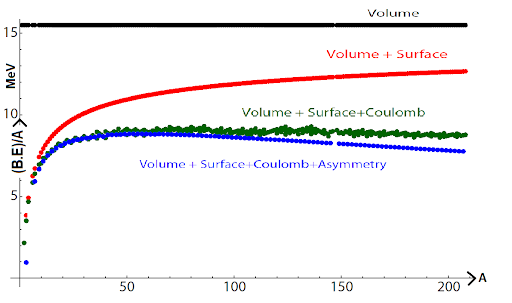
\includegraphics[width = 0.75\textwidth]{03/BE_A_plot.png}
            \caption{B(A,Z)/A plot as function of A.\\Source: MIT Open Courseware: \href{https://ocw.mit.edu/courses/nuclear-engineering/22-02-introduction-to-applied-nuclear-physics-spring-2012/}{\textit{Introduction to Applied Nuclear Physics}} by Prof. Paola Capellaro, Spring 2012.}
            \label{fig:plot_BE_A}
        \end{figure}
        
        \par In this form, the asymmetry term becomes zero when $A = 2Z$. A in the denominator ensures that this effect is less for larger $A$ and vice-versa.
        
    \item \textbf{Pairing term:}    This is the last term in the\\\textit{Bethe–Weizsäcker mass formula}. This term mimics the effect of spin-coupling. We have learned that the ground state \href{https://en.wikipedia.org/wiki/Spin_(physics)}{spin} of all the even-even nuclei are {$0\pm$} which indicates that like-nucleons tend to pair off. It means that in even-even nuclei all the neutrons and all the protons are paired which is a favourable condition to have larger binding energy. For odd-$A$ nuclei, either one proton or one neutron left out without pairing. However, for odd-odd nuclei, one proton and neutron are left unpaired and, thus, contributes least in the binding energy of a nucleus. Mathematically this effect is expressed as:
        \begin{equation}
            \begin{split}
                \delta(A,~Z)~&=~+\delta,~ \textrm       {for N and Z even (even A)}\\
                \delta(A,~Z)~&=~0,~ \textrm             {for odd A}\\
                \delta(A,~Z)~&=~-\delta,~ \textrm       {for N and Z odd (even A)}\\
            \end{split}
        \end{equation}
        
         The value of  is found to be about $1200keV$ and slowly varies with $A$ as $A^{-3/4}$.
         
        \begin{table}
                \centering
                \begin{tabular}{|c|c|}
                \hline
                unit &  MeV\\
                \hline\hline
                $a_V$ & 15.76\\[0.5em]
                $a_S$ & 17.81\\[.5em]
                $a_C$ & 0.711\\[.5em]
                $a_A$ & 23.702\\[.5em]
                $a_P$ & 34\\[.5em]
                $k_P$ & ${-3/4}$\\[.5em]
                $\delta_0$(even-even) & $\frac{+34}{A^{3/4}}$\\[1em]
                $\delta_0$(odd-odd) & $\frac{-34}{A^{3/4}}$\\[1em]
                $\delta_0$(even-odd/odd-even) & 0\\[1em]\hline
                \end{tabular}
            \caption{Experimental values of the coefficients in MeV}
            \label{tab:table_num}
        \end{table}
    
    \pagebreak\par If we add the contribution of all the terms as mentioned above, the total binding energy can be expressed as the following:
    
        \begin{equation}
            \begin{split}
                E_B (A,~Z)~=E_V~+&~E_S~+~E_C~+~E_A~+~\delta(A,~Z)\\
                E_B(A,~Z)~=~a_VA&~-~a_SA^{2/3}~-a_C\frac{Z(Z-1)}{A^{1/3}}\\
                                &~-~a_A\frac{(A-2Z)^2}{A}~+~\delta(A,~Z) 
            \end{split}
        \end{equation}    
         Contribution of each term is plotted as a function of (B.E)/A and shown in the above figure \ref{fig:plot_BE_A}. It clearly exhibits their contribution to $E_B$.
        

        
     The final relation is known as the Bethe–\\Weizsäcker mass formula (SEMF). The constants in the formula are estimated by fitting the experimental binding energy data of different nuclei from different mass regions. The values can vary depending upon the fitting methods. 
    \par The adjacent table \ref{tab:table_num} taken from \href{https://cutt.ly/VRnd6zB}{wikipedia} shows one such set of values. You may  consult the book titled \href{https://books.google.co.in/books?id=fkqHNMd_248C&lpg=PP1&pg=PP1#v=onepage&q&f=false}{\textit{Atomic and  Nuclear Physics}} by S. N. Ghosal for further discussion.     
    
\end{enumerate}




\begin{comment}
\pagebreak\section{Learning Outcome}

    \subsection{Nuclear Landscape}
        \begin{itemize}
            \item There are about 3300 nuclei known to us and around only 15\% of them are stable. Most of the unstable nuclei undergo $\beta$-decay. Most the heavy nuclei decay through  emission and few undergo spontaneous fission.
            \item In heavy nuclei, the Coulomb repulsions between the protons weaken the binding energy of a nucleus. Thus they need more neutrons to stabilize the system.
        \end{itemize}
    \subsection{Bethe–Weizsäcker Mass Formula}
        \begin{itemize}
            \item Similarities with charged liquid drop.
            \item Dissimilarities with charged liquid drop.
            \item We know that the binding energy ($E_n$) of a nucleus with atomic mass M(A, Z) may be written as \[E_B ~=~ZM_H~+NM_n~-~M(A, Z)\]
            \item The Binding energy $E_B$ is composed of the following terms:
                \begin{enumerate}[label=\textbf{\alph*.}]
                    \item Volume term
                    \item Surface term
                    \item Coulomb term
                    \item Asymmetry term
                    \item Pairing term
                \end{enumerate}
        \end{itemize}
\end{comment} 
    \chapter{{Application of Bethe-Weizsäcker Mass Formula}}

    \begin{tcolorbox} [colframe=blue!10!black,colback=yellow!29.05!white,arc=1em,fonttitle=\bfseries,title=\textit{Key Objective:}, width = \textwidth]
        $\star$ \textbf{Application of Bethe-Weizsäcker mass formula} $\star$
        \begin{itemize}
            \item Stability of a nucleus against $\alpha$-Decay 
            \item Stability of a nucleus against $\gamma$-Decay 
            \item  Mass parabola 
        \end{itemize}
    \end{tcolorbox}
    
\pagebreak\section{Stability of nucleus against $\alpha$-Decay}
    In the previous chapter we have learnt that Bethe–Weizsäcker mass formula is given by
    
     \begin{equation}
                \begin{split}
                    E_B(A,Z) =a_VA &-a_SA^{2/3} -a_C\frac{Z(Z-1)}{A^{1/3}}\\
                                    & - a_A\frac{(A-2Z)^2}{A} + \delta(A, Z)
                \end{split}
      \end{equation}    
    \par In heavy nuclei, the Coulomb repulsion becomes so strong that we need many additional
neutrons to stabilise the nucleus. It is evident from the nuclear stability line (NZ curve) which tilts
toward the N axis of the curve. It is also apparent if we study the radioactive-decay pattern of the isotopes of heavy nuclei. For
example, if we look at the most
neutron deficient and neutron rich
isotopes of
${}^{89}A$  it is quite apparent. The lighter isotopes prefer to gain stability through
decay due to greater Coulomb
repulsion whereas in heavier
isotopes, it is $\beta$-decay  which we
will learn shortly. Let us look into
the required condition of decay
as per the Bethe–Weizsäcker mass
formula.
$\alpha$-decay  decay of a nucleus, X to the daughter nucleus Y is represented as:


\pagebreak\begin{table}[ht]
        \centering
        \begin{adjustbox}{width=0.8\textwidth}
        \begin{tabular}{|l|c|c|c|}
            \hline
        \textbf{Z} & \textbf{A} & \textbf{Half-Life} & \textbf{Decay mode}\\[0.5cm]\hline
        \textbf{{89} Ac}  & {206} & {22 ms +9-5} &  {$\alpha$}\\
                       {} & {206m} & {33 ms +22-9} & {$\alpha$}\\
                       
                       {} & {207} & {27 ms +22-9} & {$\alpha$}\\
                       
                       {} & {208} & {95 ms +24-16} & {$\alpha$ $\approx99$ $\%$,$\epsilon$$\approx1$$\%$}\\[0.5em]
                       
                       {} & {208m} & {25 ms +9-5} & {$\alpha$ $\approx90$ $\%$,$\epsilon$ $\approx10$ $\%$}\\[0.5em]
                       
                       {} & {209} & {0.10 s 5} & {$\alpha\approx99\%,\epsilon \approx1\%$}\\[0.5em]
                       
                       {} & {210} & {0.35 s 5} & {$\alpha\approx91\%,~\epsilon \approx9$\%}\\[0.5em]
                       
                       {} & {211} & {0.21 s 3} & {$\alpha$}\\
                       
                       {} & {212} & {0.93 s 5} & {$\alpha\approx57\%,~\epsilon \approx43\%$ }\\[0.5em]
                       
                       {} & {227} & {21.772 y 3} & {$\beta\approx$- 98.62$\%$, $\alpha\approx$ 1.38$\%$}\\[0.5em]
                  
                       {} & {228} & {6.15 h 2} & {$\beta$-}\\
                       
                       {} & {229} & {62.7 m 5} & {$\beta$-}\\
                       
                       {} & {230} & {122 s 3} & {$\beta$-,~$\beta-\approx~ 1.2*10^-6\% $}\\[0.5em]
                       
                       {} & {231} & {7.5 3 1} & {$\beta$-}\\
                       
                       {} & {232} & {119 s 5} & {$\beta$-}\\
                       
                       {} & {233} & {145 s 10} & {$\beta$-}\\
                       
                       {} & {234} & {44 s 7} & {$\beta$-}\\
                       
                       {} & {235} & {60 s 4} & {$\beta$-}\\
                       
                       \hline
                  
        \end{tabular}            
        \end{adjustbox}

 \label{tab:table_decaymode}
\caption{Half-life and decay mode of nine most lightest and heaviest isotopes of Actinum(Ac).}
 \end{table}
    \begin{equation}
   {}^{A}_{Z}X  \longrightarrow {}^{A-4}_{Z-2}Y +{}^{4}_{2}He(\alpha)
     \end{equation}

We have learned to calculate the disintegration energy Q as follows,
\begin{equation}
Q_\alpha=M(A,Z)- M(A-4,Z-2)-M_\alpha
\end{equation}

Since total numbers of neutrons and protons are constants, if we substitute the M’s according
to the binding energy formula $E_B=ZM_H+NM_n-M(A, Z)$
it gives us,
\begin{equation}
Q_\alpha=E_B(A-4,Z-2)+E_B(\alpha)-E_B(A,Z)
\end{equation}   
   
 Using the Bethe–Weizsäcker mass formula, we can rewrite the above equation
\begin{multline}
Q_\alpha=a_V(A-4)-a_S(A-4)^{2/3}-a_C\frac{(Z-2)}{(A-4)^{1/3}}-a_A\frac{(A-2Z)^2}{(A-4)}\\
~-a_VA+a_SA^{2/3}+\frac{Z^2}{A^{1/2}}+a_A\frac{(A-2Z)^2}{A}+E_B(\alpha)
\end{multline} 

 
\par We have replaced Z(Z-1) as $Z^2$.  The total binding energy of $\alpha$ particle is 28.3 MeV. Thus,
  \begin{equation}
  Q_\alpha=28.34a_V+a_S\frac{8/3}{A^{-1/3}}+a_C\frac{4Z}{A^{1/2}}(1-\frac{Z}{3A})-a_A\frac{4(A-2Z)^2}{A(A-4)}
  \end{equation}

If we replace the proportionality constants (a’s) with their estimated values, the $Q_\alpha>0$  (condition to occur $\alpha$-decay) for $A>160$ which is close to the experimental value.


   
\pagebreak\section{{Stability of nucleus against $\beta$-Decay}}
 
\subsection{The Mass Parabola and stability:}
   The Bethe–Weizsäcker mass formula is a function of A and Z. Therefore, it gives us the opportunity to study
the behaviour of M(A, Z) as a function of Z. It will
help us find out the most stable Z value for nuclei
with a fixed A (i.e. isobar: nuclei with same mass
number A). We rewrite the mass formula as a
function of Z as,
\begin{equation}
\begin{split}
     M(A, Z)=K_1+K_2Z+K_3Z^2{\pm}\delta
\\ \textrm where,
\\\textrm K1=A(M_n-a_V+a_A+a_S^{-1/3}),
 \\\textrm K2=-[4a_A+(M_n-M_H)],
  \\ \textrm K3=(4\frac{a_A}{A}+\frac{a_C}{A^{1/3}}).
\end{split}
\end{equation}
 
\par Since $\delta$ is independent of A, we may neglect it.
The variation of M(A, Z) takes the form of a parabola for a given A. For a particular Z value, M(A,Z) reaches the minimum of the curve and it corresponds to the most stable nucleus for that A.The adjoining figure is showing a representative mass parabola for A=135 (Source: MIT OCW,
22.101 Applied Nuclear Physics, Fall 2006). The most stable nucleus $(Z_A)$  for this mass number is ${}^{56}B $.

     We can obviously calculate it as 
\begin{align}
\frac{\delta M(A,Z)}{\delta Z}=0=K_2+2k_3Z_A\\
\textrm{So,}
~~Z_A= -\frac{K_2}{2K_3}=\frac{(M_n-M_H+4a_A)A}{2(a_cA^2/3+4a_A)}
\end{align}
     
If we substitute $Z_A$ in the expression of M(A,Z), we get 
\begin{equation}
 \begin{split}
 M(A,Z_A)=K_1+K_2&(-K_2/2K_3)+K_3\frac{K_2^2}{4K_3^2}=K_1-\frac{K_2^2}{4k_3}\\
\textrm{So,}~~M(A,Z_A)-M(A,&~Z_A)=\frac{K_2^2}{4K_3^2}+K_2Z+K_3Z^2\\&=K_3(Z^2-2Z_AZ+Z_A^2)\\
\therefore M(A,Z)-&M(A,Z_A)=K_3(Z-Z_A)^2 
\end{split}  
\end{equation} 

   
It shows that at $Z=Z_A$ , a mass parabola reaches its minima for a given A value. It gives an approximate value of the transition energies in $\beta$-decay reactions. The usefulness of the above exercise can be appreciated in many ways. Let us substitute the values of $M_n, M_H, a_C $ and $a_A $ and we get
  \begin{equation}
  Z_A=\frac{A}{1.98+0.015A^{2/3}}
   \end{equation}
   
  For a given A, the above expression provides a fairly accurate estimate of the corresponding $Z_A$.For example, if we replace A with 63, the corresponding $Z_A = 28.4$. Experimentally the most stable nucleus for A=63 is Cu (Z=29).The expression for also gives us an idea of the effect of Coulomb force. If we neglect the asymmetry term is that expression, it becomes,
  \begin{equation}
  Z_A=\frac{(M_n-M_H)A}{2a_CA^{2/3}}=\approx-.9A^{1/3}
      \end{equation}

For Z=18, A is 8000 which is unrealistic! It clearly demonstrates that the Coulomb force is really responsible for observation of the deviation of the line of stability from the N=Z line.

\begin{wrapfigure}{l}{0.5\textwidth}
         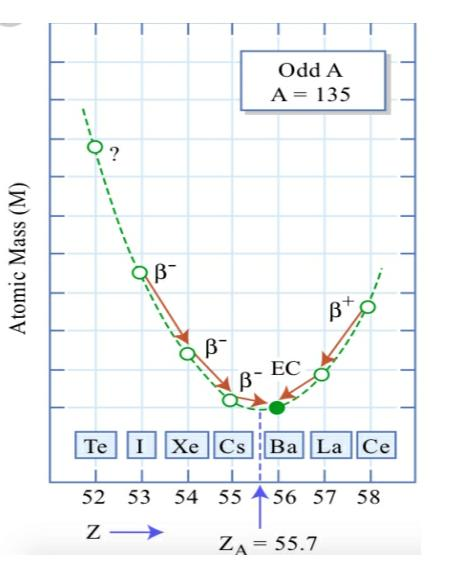
\includegraphics[width =0.48\textwidth]{04/ZVM_plot.jpg}
         \caption{Z vs M Plot(for odd A)}
         \label{fig:plot_ZvsM}
\end{wrapfigure}
     
\subsection{Stability of a nucleus against $\beta$-decay:}   The obvious question might have come to your mind “what will happen to the other nuclei of the mass parabola away from $Z_A $ ?”. Actually this question answers one of the most important aspects of the mass parabola: The origin of $\beta$ instability or the origin of $\beta$-decay. The only way to reach the minima of the mass parabola without changing A value is to undergo $\beta$-decay. The nuclei away from with $Z > Z_A$ undergo $\beta^-$ decay. It is represented as
     \begin{equation}
        {}^{A}_{Z}X  \longrightarrow {}^{A}_{Z+1}Y  + \beta^-+\gamma 
      \end{equation}
      
\begin{wrapfigure}{r}{0.5\textwidth}
    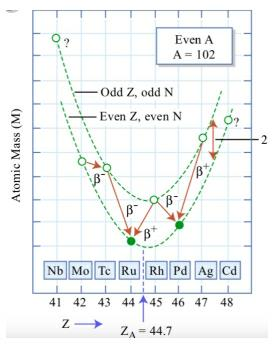
\includegraphics[width=0.48\textwidth]{04/ZVA_plot.jpg}
    \caption{Z vs M plot (for even A)}
    \label{fig:plot_ZvsM2}
\end{wrapfigure}

\par $\gamma$ is a nearly massless, chargeless fermion and $\gamma$ is the anti-neutrino. We will discuss it in due course of time. In the above mass parabola picture, the nuclei Te, I, Xe, and Cs are going through successive
$\beta^-{}$ decay to increase their Z value until ${}^{135}B $ is reached.

Similarly, nuclei with $ Z > Z_A $ undergo decay to decrease their Z values to reach the minima. A typical $\beta^+{}$ decay to reach the minima.
\begin{equation}
  {}^{A}_{Z}X \longrightarrow {}^{A}_{Z-1}Y  + \beta^+ + \gamma
\end{equation}

 In the above figure, Ce and La undergo repeated $\beta^+$ decay to reach the minima.
 
 It is interesting to note that in case of even-A nuclei,there are two possibilities; a) both N and Z are odd (odd-odd) and b) both N and Z are even (even-even).In the first -$\delta$ case and for the later case, it is +$\delta$ .Therefore, we get two mass parabolas instead of one with their minima shifted by . The adjoining figure \ref{fig:plot_ZvsM2}
({\textit{\textbf{Source:} MIT OCW, 22.101 Applied Nuclear Physics, Fall 2006}})
clearly demonstrates this fact.



One thing should be mentioned that few nuclei undergo double $\beta$-decay. In ordinary double $\beta$-decay, two neutrons are converted into protons inside the nucleus. Two electrons and two electron type $\gamma$ are emitted. However, only very few nuclei (14
nuclei between ${}^{48}Ca $ and ${}^{238}U $) have shown double $\beta$-decay. It will only be possible, if the final nucleus has greater binding energy than the original nucleus. One example is ${}^{76}Ge $ .The most stable for A=76 isobars is ${}^{76}Se $ . The ${}^{76}Ge $ should undergo a $\beta^-$-decay  and form $^{76}As$ which in turn perform another  $\beta^-$-decay to reach the minima at ${}^{76}Se $ . However, $^{76}As$ has a smaller binding energy than ${}^{76}Ge $ which prevents the single $\beta^-$-decay. The ${}^{76}Se $ , on the other hand, has larger binding energy which allows the ${}^{76}Ge $ to go through double $\beta$-decay. Conceptually it is possible to have neutrinoless double $\beta^-$-decay where only electrons would be emitted. However, experimentally it is yet to be observed.
    
%----------------------------------------------------------------------------------------------------------
\renewcommand{\footrulewidth}{0.25pt}
\thispagestyle{the_end} 

\end{document}